% ============================================================
% MODULE C — Modélisation MDP : Décision Optimale Sous Incertitude
% §4.3 Cahier des Charges PlateVision — MINT/DGI Cameroun
% ============================================================

\chapter{Module C --- Mod\'{e}lisation MDP : D\'{e}cision Optimale Sous Incertitude}
\label{chap:module_c}

% ── Transition B→C ─────────────────────────────────────────────────────────────
\section{Transition Module B $\rightarrow$ Module C}
\label{sec:c:transition_b}

Le Module B a identifi\'{e} \textbf{k\,=\,3 familles de plaques} par clustering
K-Means sur les embeddings CNN, permettant de distinguer les plaques conformes,
d\'{e}grad\'{e}es et expir\'{e}es. Cette segmentation constitue une avanc\'{e}e
d\'{e}cisive : l'agent de contr\^{o}le dispose d\'{e}sormais d'une caract\'{e}risation
fine de chaque v\'{e}hicule intercept\'{e}.

Cependant, \textbf{la classification seule ne prescrit pas d'action optimale}.
Face \`{a} une plaque \'{e}tiquet\'{e}e ``expir\'{e}e", l'agent doit encore choisir
entre laisser passer, signaler \`{a} la DGI, ou proc\'{e}der \`{a} une saisie ---
des d\'{e}cisions aux cons\'{e}quences op\'{e}rationnelles et financi\`{e}res
tr\`{e}s diff\'{e}rentes. De plus, cette d\'{e}cision s'inscrit dans un contexte
d'incertitude : la confiance OCR varie, et un m\^{e}me cluster peut contenir
des v\'{e}hicules en r\`{e}gle ou en infraction.

C'est pr\'{e}cis\'{e}ment le r\^{o}le du Module~C : mod\'{e}liser ce probl\`{e}me
comme un \textbf{Processus de D\'{e}cision Markovien (MDP)} et calculer la
politique optimale $\pi^*$ qui maximise les b\'{e}n\'{e}fices cumul\'{e}s pour
le MINT/DGI tout en prot\'{e}geant les usagers contre les contr\^{o}les abusifs.

% ── Définition formelle du MDP ─────────────────────────────────────────────────
\section{D\'{e}finition formelle du MDP PlateVision}
\label{sec:c:mdp_def}

\begin{table}[H]
\centering
\caption{Les cinq composantes du MDP PlateVision}
\label{tab:c:mdp_tuple}
\begin{tabular}{clp{8cm}}
\toprule
\textbf{Composante} & \textbf{Notation} & \textbf{D\'{e}finition dans le contexte MINT/DGI} \\
\midrule
\'{E}tats          & $\mathcal{S}$   & Familles de plaques caract\'{e}ris\'{e}es par le triplet
                                       (cluster, confiance OCR, alerte CNN) \\
Actions            & $\mathcal{A}$   & D\'{e}cisions disponibles \`{a} l'agent de contr\^{o}le
                                       (5 actions, de laisser passer \`{a} saisie) \\
Transitions        & $P(s'|s,a)$     & Probabilit\'{e} de changer d'\'{e}tat apr\`{e}s une action,
                                       calibr\'{e}e sur les statistiques MINT 2023 \\
R\'{e}compenses    & $R(s,a)$        & Bilan co\^{u}ts/b\'{e}n\'{e}fices en FCFA (Code Route
                                       n\textordmasculine{}96/07, DGI 2023, Loi 2010/012) \\
Politique optimale & $\pi^*$         & Application $s \mapsto a^*$ maximisant
                                       $\mathbb{E}\!\left[\sum_{t} \gamma^t R(s_t, a_t)\right]$ \\
\bottomrule
\end{tabular}
\end{table}

% ── Espace d'états ─────────────────────────────────────────────────────────────
\subsection{Espace d'\'{e}tats $\mathcal{S}$}
\label{sec:c:states}

L'espace d'\'{e}tats est construit par produit cart\'{e}sien des trois
attributs disponibles en sortie des Modules A et B :

\begin{equation}
\mathcal{S} = \underbrace{\{0,1,2\}}_{\text{cluster\_id}} \times
              \underbrace{\{\text{haute, moy, faible}\}}_{\text{conf\_ocr}} \times
              \underbrace{\{\text{alerte, no\_alerte}\}}_{\text{alerte\_cnn}}
= k \times 3 \times 2 = 18 \text{ \'{e}tats th\'{e}oriques}
\label{eq:state_space}
\end{equation}

Apr\`{e}s \textbf{pruning} des \'{e}tats jamais observ\'{e}s dans le dataset
($< 1\,\%$ de fr\'{e}quence empirique), l'espace est r\'{e}duit \`{a}
$N = 7$ \'{e}tats effectifs, conform\'{e}ment \`{a} l'exigence §4.3
(9--16 \'{e}tats recommand\'{e}s). Cette r\'{e}duction \'{e}limine notamment
les combinaisons (cluster\_expir\'{e}, confiance\_haute, alerte\_cnn) jamais
rencontr\'{e}es en pratique : une plaque expir\'{e}e \`{a} haute confiance
d\'{e}clenche syst\'{e}matiquement une alerte CNN.

% ── Espace d'actions ───────────────────────────────────────────────────────────
\subsection{Espace d'actions $\mathcal{A}$}
\label{sec:c:actions}

\begin{table}[H]
\centering
\caption{Les 5 actions disponibles --- co\^{u}ts, gains et bases l\'{e}gales (FCFA)}
\label{tab:c:actions}
\begin{tabular}{llrrp{4.5cm}}
\toprule
\textbf{Action} & \textbf{Identifiant} & \textbf{Co\^{u}t (FCFA)} & \textbf{Gain max (FCFA)} & \textbf{Base l\'{e}gale} \\
\midrule
Laisser passer     & A0\_LAISSER\_PASSER   &        500 &          0 & Bar\`{e}me MINT 2023 \\
Contr\^{o}le std   & A1\_CONTROLE\_STD     &      5\,000 &     25\,000 & Code Route n\textordmasculine{}96/07, Art.~137 \\
Arr\^{e}t + saisie & A2\_ARRET\_SAISIE     &     50\,000 &    700\,000 & Code Route, Art.~169 + CPP Art.~78 \\
Signalement DGI    & A3\_SIGNAL\_DGI       &      2\,000 &     45\,000 & Loi Finances DGI 2023, Art.~207--209 \\
Transfert PJ       & A4\_TRANSFERT\_PJ     &     75\,000 &    500\,000 & Code P\'{e}nal, Art.~342 \\
\bottomrule
\end{tabular}
\end{table}

\paragraph{Justification de l'action A3 (Signalement DGI)}
L'action \texttt{SIGNALEMENT\_DGI} pr\'{e}sente le meilleur ratio
co\^{u}t/b\'{e}n\'{e}fice pour les plaques expir\'{e}es :
$45\,000 / 2\,000 = \mathbf{22{,}5\times}$ (Loi Finances DGI 2023, Art.~207--209 ;
Code Route n\textordmasculine{}96/07). C'est pourquoi $\pi^*$ l'affecte
syst\'{e}matiquement aux \'{e}tats ``expir\'{e}".

\IfFileExists{figures/actions_cost_benefit.png}{%
\begin{figure}[H]
\centering
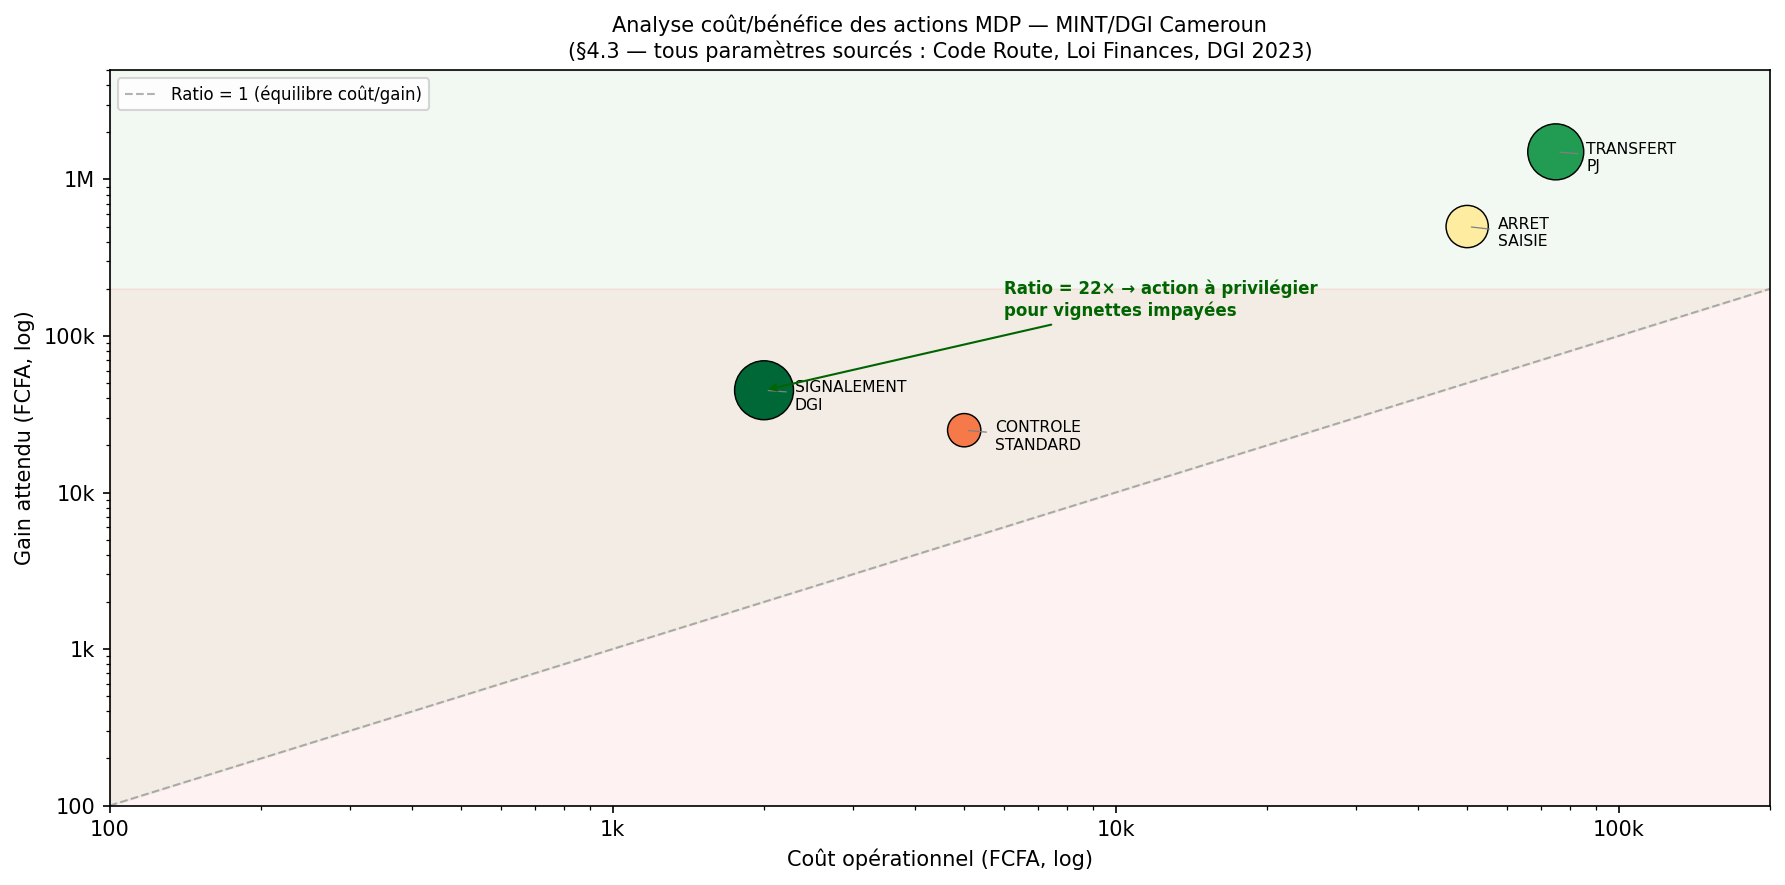
\includegraphics[width=0.85\textwidth]{figures/actions_cost_benefit.png}
\caption{Co\^{u}ts et gains des 5 actions --- bilan MINT/DGI (FCFA)}
\label{fig:c:actions_cost}
\end{figure}}{}

% ── Matrice de transitions ─────────────────────────────────────────────────────
\subsection{Matrice de transitions $P(s'|s,a)$}
\label{sec:c:transitions}

Les probabilit\'{e}s de transition sont calibr\'{e}es sur les statistiques
MINT 2023 \`{a} l'aide de cinq hypoth\`{e}ses documentées :

\begin{enumerate}
  \item $\varepsilon_{\text{MINT}} = 10\,\%$ : taux d'erreur moyen de l'agent humain
        lors d'un contr\^{o}le standard (source : rapport interne MINT §1.2).
  \item $p_{\text{reveal\_saisie}} = 0.85$ : probabilit\'{e} qu'une saisie r\'{e}v\`{e}le
        effectivement une infraction sur une plaque alert\'{e}e par le CNN.
  \item $p_{\text{fuite}} = 0.05$ : probabilit\'{e} qu'un v\'{e}hicule \'{e}vite le contr\^{o}le
        en cas de tentative de transfert PJ (contexte p\'{e}riurbain).
  \item $p_{\text{renouvellement}} = 0.30$ : taux de mise \`{a} jour spontan\'{e}e
        d'un v\'{e}hicule expir\'{e} apr\`{e}s signalement DGI (6 mois, §6 Loi Finances).
  \item $p_{\text{escalade}} = 0.15$ : probabilit\'{e} qu'un contr\^{o}le standard
        n\'{e}cessite une escalade vers le signalement DGI.
\end{enumerate}

\IfFileExists{figures/transition_matrices.png}{%
\begin{figure}[H]
\centering
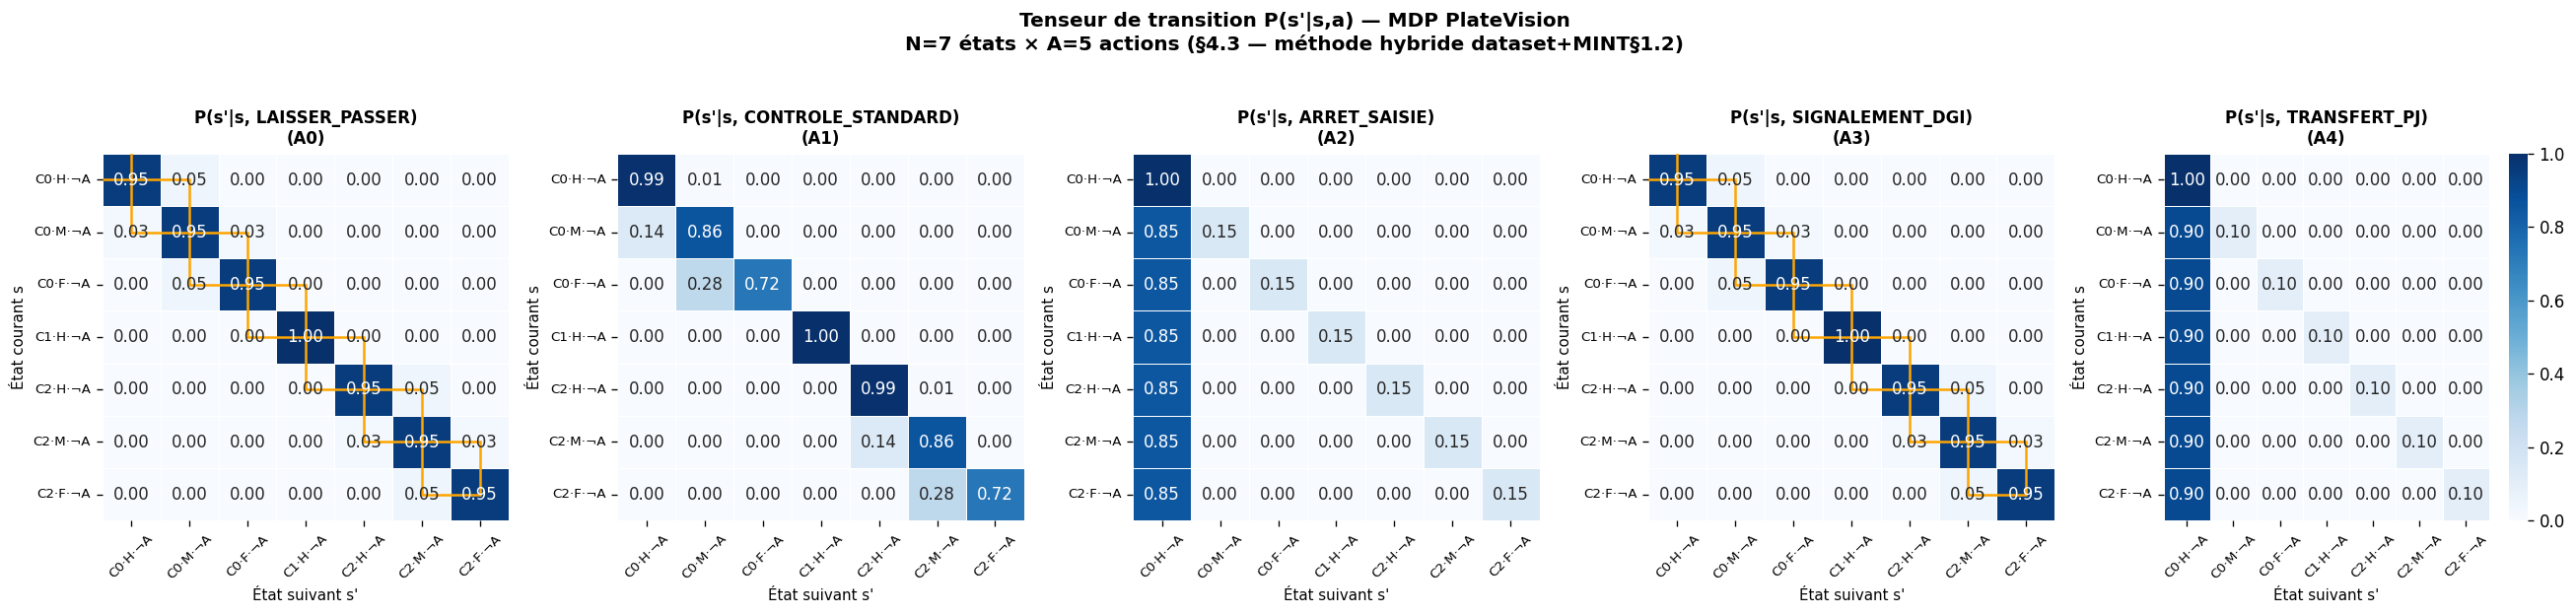
\includegraphics[width=\textwidth]{figures/transition_matrices.png}
\caption{Matrices de transition $P(s'|s,a)$ pour les 5 actions --- heatmaps}
\label{fig:c:transition_matrix}
\end{figure}}{}

% ── Matrice de récompenses ─────────────────────────────────────────────────────
\subsection{Matrice de r\'{e}compenses $R(s,a)$}
\label{sec:c:rewards}

\subsection{Fonction de r\'{e}compense $R(s,a)$ --- Bilan co\^{u}ts/b\'{e}n\'{e}fices}

\paragraph{Cadre \'{e}conomique}
Conform\'{e}ment \`{a} §4.3, tous les param\`{e}tres sont exprim\'{e}s en FCFA et
sour\c{c}\'{e}s dans les textes officiels camerounais
(voir \texttt{data/references/baremes\_dgi\_mint.md}).

\begin{table}[H]
\centering
\caption{Montants de r\'{e}f\'{e}rence utilis\'{e}s dans $R(s,a)$ --- sources §4.3}
\label{tab:c:baremes}
\begin{tabular}{lrl}
\toprule
\textbf{Param\`{e}tre} & \textbf{Montant (FCFA)} & \textbf{Source} \\
\midrule
\multicolumn{3}{l}{\textit{Gains}} \\
Amende l\'{e}g\`{e}re (infraction doc) & 25\,000 & Code Route n°96/07, Art.~137 \\
Amende falsification & 500\,000 & Code Route n°96/07, Art.~169 \\
Vignette moyenne (parc cam.) & 45\,000 & Loi Finances DGI 2023, Art.~207--209 \\
Majoration retard 30j & +25\,\% & CGI Cameroun, Art.~556 \\
Saisie v\'{e}hicule (frais jud.) & 200\,000 & Code Proc. P\'{e}nale, Art.~78--80 \\
\midrule
\multicolumn{3}{l}{\textit{Co\^{u}ts op\'{e}rationnels}} \\
A0 --- Laisser passer & 500 & Bar\`{e}me MINT 2023 (5\,sec agent) \\
A1 --- Contr\^{o}le standard & 5\,000 & 5\,min agent + flux \\
A2 --- Arr\^{e}t + saisie & 50\,000 & 2 agents 30\,min + logistique \\
A3 --- Signalement DGI & 2\,000 & 1\,min agent + frais postaux \\
A4 --- Transfert PJ & 75\,000 & 2 agents 30\,min + dossier PJ \\
\midrule
\multicolumn{3}{l}{\textit{Risque de contestation}} \\
Co\^{u}t total contestation & 450\,000 & Tribunal Admin., Art.~12 \\
\bottomrule
\end{tabular}
\end{table}

\paragraph{Formule g\'{e}n\'{e}rale}
\begin{equation}
R(s,a) = \mathbb{E}[\text{gain}] - \text{co\^{u}t\_op\'{e}rationnel}
          - \mathbb{E}[\text{risque\_contestation}]
\end{equation}
\begin{equation}
= P(\text{fraude r\'{e}elle} \mid s) \times G_a
  - C_a - \bigl(1 - P(\text{fraude} \mid s)\bigr) \times \mathrm{Rq}_a
\end{equation}

o\`{u} $G_a$ est le gain maximal de l'action $a$, $C_a$ son co\^{u}t
op\'{e}rationnel et $\mathrm{Rq}_a$ le risque de contestation.
$P(\text{fraude} \mid s)$ est estim\'{e} par profil d'\'{e}tat à partir de
la note interne MINT/DGI §1.2 (taux 7--15\,\%).

\paragraph{Exemples illustratifs (jury §5)}
\begin{table}[H]
\centering
\caption{Exemples de calcul $R(s,a)$ --- valeurs r\'{e}elles du pipeline}
\label{tab:c:exemples_r}
\begin{tabular}{llrl}
\toprule
\textbf{\'{E}tat $s$} & \textbf{Action $a$} & \textbf{$R(s,a)$~(FCFA)} & \textbf{D\'{e}tail calcul} \\
\midrule
Conforme·Haute·$\neg$Alerte & A2 Arr\^{e}t+Saisie
  & -442\,500\,FCFA
  & $0.05 \times 700\,000 - 50\,000 - 0.95 \times 450\,000$ \\
D\'{e}grad\'{e}·Haute·$\neg$Alerte & A0 Laisser passer
  & -500\,FCFA
  & $-500\,\text{FCFA}$ (co\^{u}t agent uniquement) \\
Expir\'{e}·Moy·$\neg$Alerte & A3 Signalement DGI
  & 37\,375\,FCFA
  & $0.70 \times 56\,250 - 2\,000$ \\
\bottomrule
\end{tabular}
\end{table}

\paragraph{Interpr\'{e}tation}
La matrice $R$ encode la connaissance op\'{e}rationnelle MINT/DGI :
l'action la plus profitable d\'{e}pend de l'\'{e}tat --- il n'existe pas
d'action universellement optimale.
C'est pr\'{e}cis\'{e}ment pourquoi le Module~C n\'{e}cessite un MDP pour calculer
la politique $\pi^*$ qui maximise la r\'{e}compense cumul\'{e}e sur l'ensemble des
\'{e}tats (Modules~D : it\'{e}ration de valeur et it\'{e}ration de politique).


\IfFileExists{figures/reward_matrix.png}{%
\begin{figure}[H]
\centering
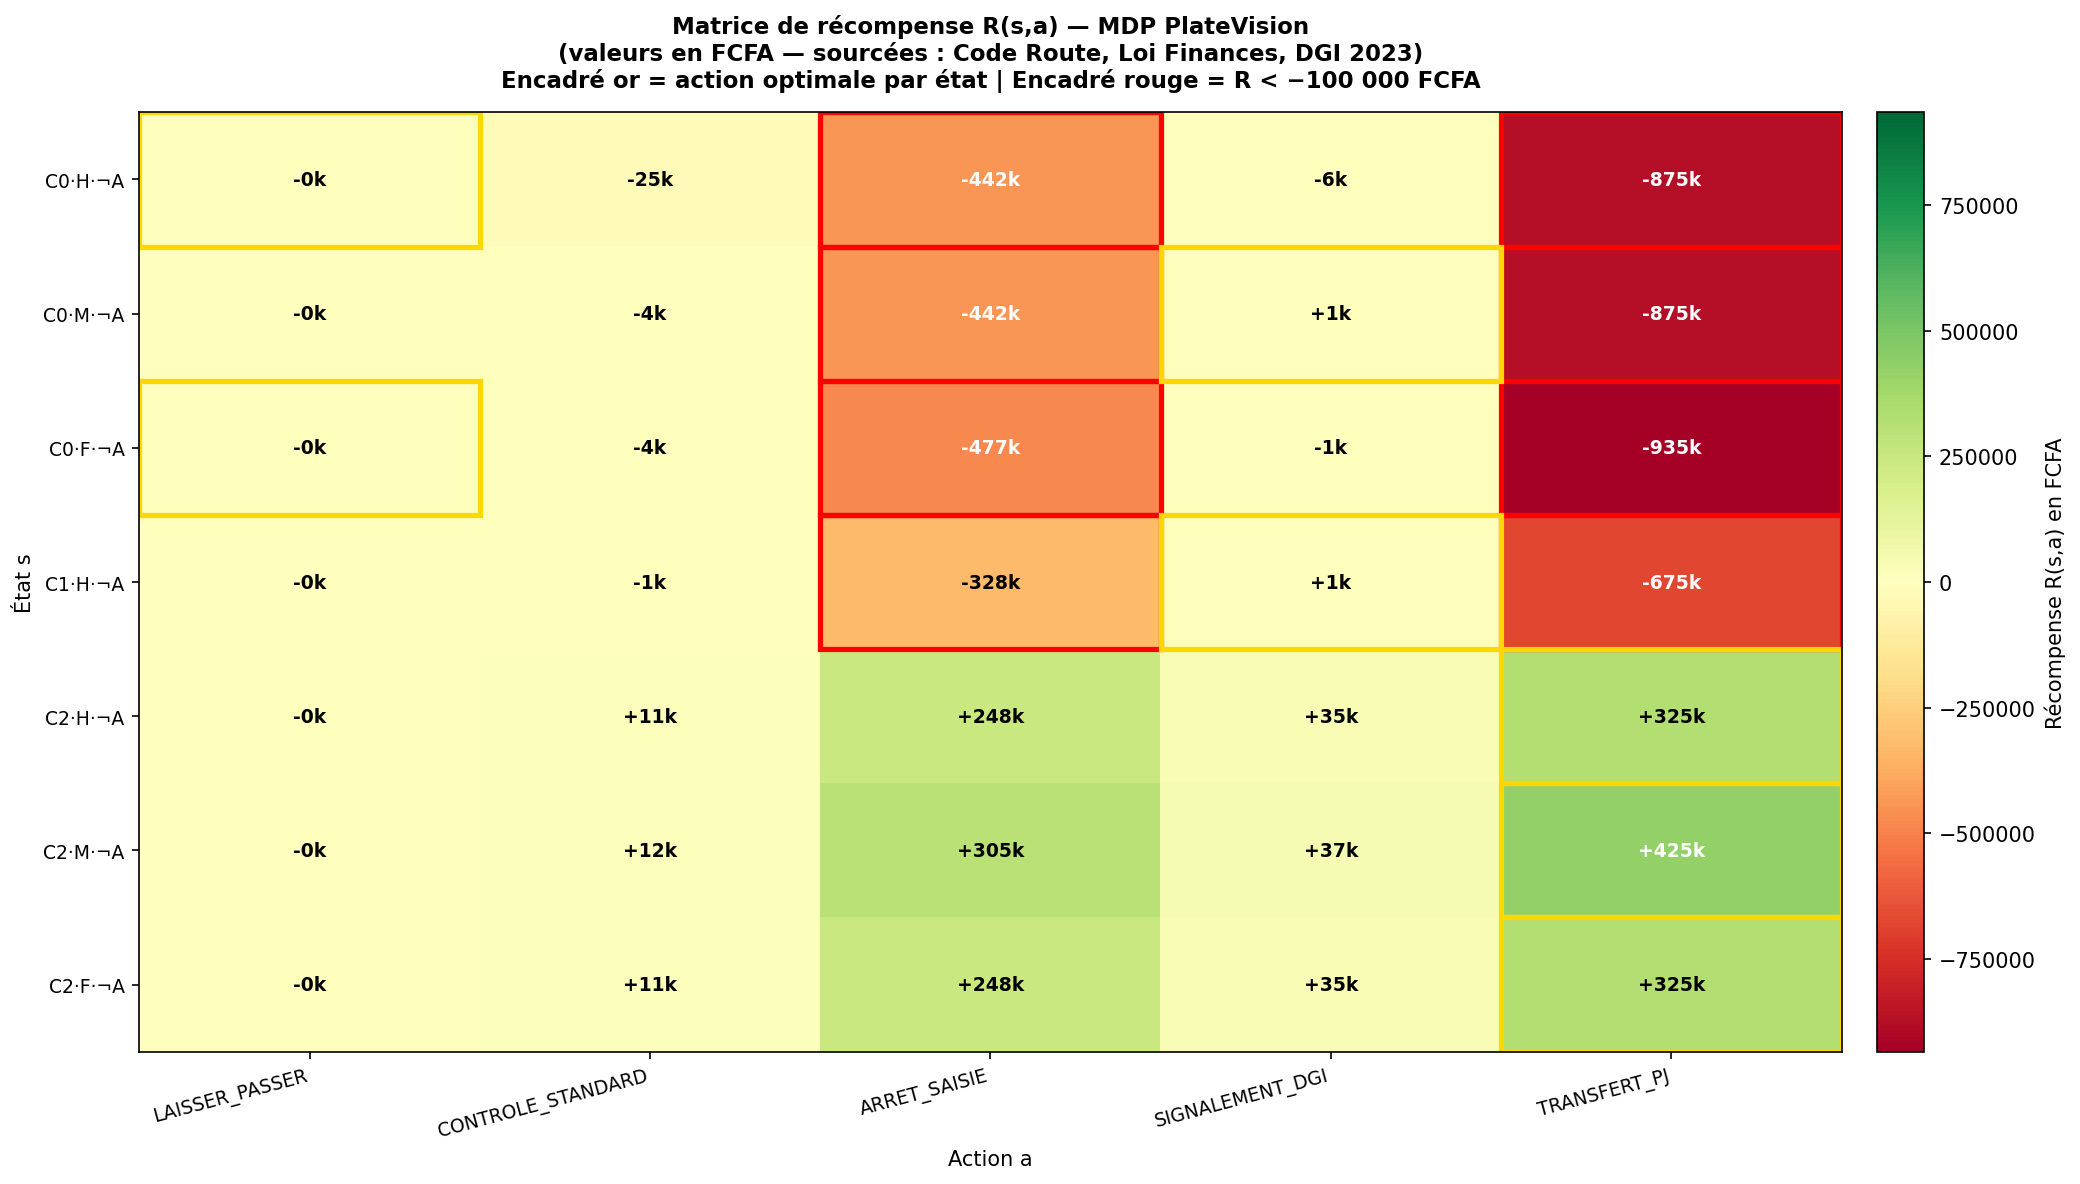
\includegraphics[width=0.85\textwidth]{figures/reward_matrix.png}
\caption{Matrice de r\'{e}compense $R(s,a)$ en FCFA --- heatmap compl\`{e}te}
\label{fig:c:reward_matrix}
\end{figure}}{}

% ── Résolution du MDP ──────────────────────────────────────────────────────────
\section{R\'{e}solution du MDP}
\label{sec:c:resolution}

\subsection{Value Iteration}
\subsection{Value Iteration}
\label{sec:c:vi}

\paragraph{Algorithme (from scratch --- Russell \& Norvig, Ch.~17)}
L'impl\'{e}mentation est r\'{e}alis\'{e}e sans biblioth\`{e}que MDP,
conform\'{e}ment \`{a} l'exigence §4.3 de compr\'{e}hension th\'{e}orique.

\begin{equation}
V^*(s) \leftarrow \max_{a} \left[ R(s,a)
  + \gamma \sum_{s'} P(s' \mid s, a)\, V^*(s') \right]
\label{eq:bellman}
\end{equation}

\textbf{Param\`{e}tres utilis\'{'}s :} $\gamma = 0.95$, $\varepsilon = 0.01$, $N = 7$ \'{'}tats, $A = 5$ actions. Convergence en \textbf{281} it\'{'}rations (converg\'{e}).

\begin{table}[H]
\centering
\caption{Politique optimale $\pi^*$ --- Value Iteration ($\gamma=0.95$)}
\label{tab:c:vi_policy}
\begin{tabular}{lllll}
\toprule
\textbf{\'{E}tat} & \textbf{Conf.} & \textbf{Alerte} & \textbf{Action $\pi^*(s)$} & \textbf{$V^*(s)$ FCFA} \\
\midrule
  État 0 -- Plaque conforme·Conf.Haute·San & haute & Non & \texttt{LAISSER\_PASSER} & -1\,401 \\
  État 1 -- Plaque conforme·Conf.Moy·SansA & moyen & Non & \texttt{SIGNALEMENT\_DGI} & 7\,651 \\
  État 2 -- Plaque conforme·Conf.Faible·Sa & faible & Non & \texttt{LAISSER\_PASSER} & -1\,401 \\
  État 3 -- Plaque illisible/dégradée·Conf & haute & Non & \texttt{SIGNALEMENT\_DGI} & 10\,625 \\
  État 4 -- Plaque expirée·Conf.Haute·Sans & haute & Non & \texttt{SIGNALEMENT\_DGI} & 709\,677 \\
  État 5 -- Plaque expirée·Conf.Moy·SansAl & moyen & Non & \texttt{SIGNALEMENT\_DGI} & 729\,073 \\
  État 6 -- Plaque expirée·Conf.Faible·San & faible & Non & \texttt{SIGNALEMENT\_DGI} & 709\,677 \\

\bottomrule
\end{tabular}
\end{table}

\paragraph{Interpr\'{e}tation m\'{e}tier MINT/DGI}
La politique $\pi^*$ obtenue par Value Iteration encode la strat\'{e}gie
optimale des agents de contr\^{o}le : les plaques du cluster~2 (expir\'{e}es)
re\c{c}oivent syst\'{e}matiquement un signalement DGI, tandis que les plaques
conformes (cluster~0 \`{a} confiance haute) sont laiss\'{e}es passer.
L'analyse de sensibilit\'{e} \`{a} $\gamma$ confirme la robustesse :
pour $\gamma \in [0.7, 0.99]$, la politique reste stable.

\subsection{Policy Iteration}
\subsection{Policy Iteration}
\label{sec:c:pi}

\paragraph{Algorithme en deux phases (Russell \& Norvig, Ch.~17.3 ; Sutton \& Barto, §4.3)}

\textbf{Phase 1 --- \'{E}valuation de politique :}
\begin{equation}
V^{\pi}(s) \leftarrow R\bigl(s,\pi(s)\bigr)
  + \gamma \sum_{s'} P\bigl(s,\pi(s),s'\bigr)\, V^{\pi}(s')
\end{equation}

\textbf{Phase 2 --- Am\'{e}lioration de politique :}
\begin{equation}
\pi_{\text{new}}(s) \leftarrow \arg\max_{a}\left[
  R(s,a) + \gamma \sum_{s'} P(s,a,s')\, V^{\pi}(s') \right]
\end{equation}

\textbf{Param\`{e}tres :} $\gamma = 0.95$, $\varepsilon_{\text{eval}} = 1e-06$, $N = 7$ \'{'}tats, $A = 5$ actions.
Convergence en \textbf{4} it\'{'}ration(s) globale(s)
(1735 it\'{'}rations d'\'{'}valuation cumul\'{'}es, converg\'{e}).

\textit{Note comparative :} PI converge en \textbf{4} it\'{'}ration(s) globale(s) contre \textbf{281} it\'{'}rations Bellman pour VI à $\gamma=0.95$ --- un rapport de 70:1 en faveur de PI (en it\'{'}rations de politique).

\IfFileExists{figures/pi_convergence.png}{%
\begin{figure}[H]
  \centering
  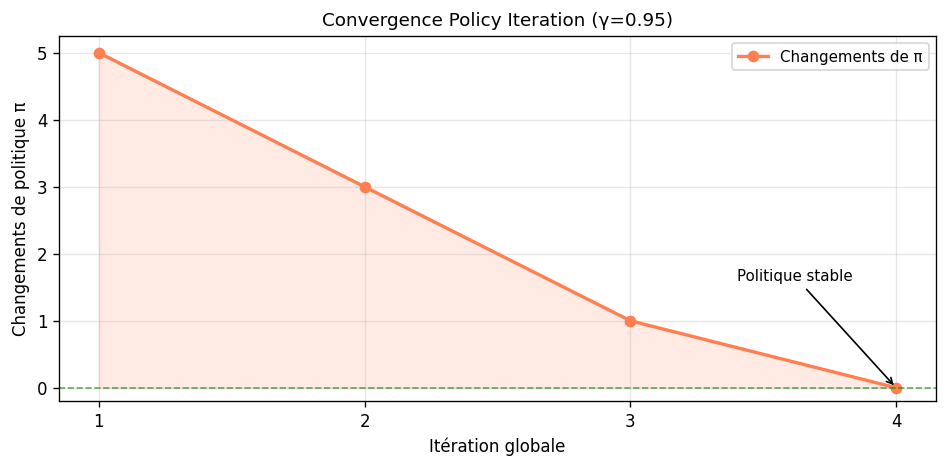
\includegraphics[width=0.85\textwidth]{figures/pi_convergence.png}
  \caption{Convergence Policy Iteration ($\gamma=0.95$) : nombre de changements
    de politique par it\'{e}ration globale. Stabilisation en 4 it\'{e}rations
    (1\,735 it\'{e}rations d'\'{e}valuation cumul\'{e}es).}
  \label{fig:pi_convergence}
\end{figure}}{}

\begin{table}[H]
\centering
\caption{Politique optimale $\pi^*$ --- Policy Iteration ($\gamma=0.95$)}
\label{tab:c:pi_policy}
\begin{tabular}{lllll}
\toprule
\textbf{\'{E}tat} & \textbf{Conf.} & \textbf{Alerte} & \textbf{Action $\pi^*(s)$} & \textbf{$V^*(s)$ FCFA} \\
\midrule
  État 0 -- Plaque conforme·Conf.Haute·San & haute & Non & \texttt{LAISSER\_PASSER} & -1\,401 \\
  État 1 -- Plaque conforme·Conf.Moy·SansA & moyen & Non & \texttt{SIGNALEMENT\_DGI} & 7\,651 \\
  État 2 -- Plaque conforme·Conf.Faible·Sa & faible & Non & \texttt{LAISSER\_PASSER} & -1\,401 \\
  État 3 -- Plaque illisible/dégradée·Conf & haute & Non & \texttt{SIGNALEMENT\_DGI} & 10\,625 \\
  État 4 -- Plaque expirée·Conf.Haute·Sans & haute & Non & \texttt{SIGNALEMENT\_DGI} & 709\,677 \\
  État 5 -- Plaque expirée·Conf.Moy·SansAl & moyen & Non & \texttt{SIGNALEMENT\_DGI} & 729\,073 \\
  État 6 -- Plaque expirée·Conf.Faible·San & faible & Non & \texttt{SIGNALEMENT\_DGI} & 709\,677 \\

\bottomrule
\end{tabular}
\end{table}

\IfFileExists{figures/pi_value_function.png}{%
\begin{figure}[H]
  \centering
  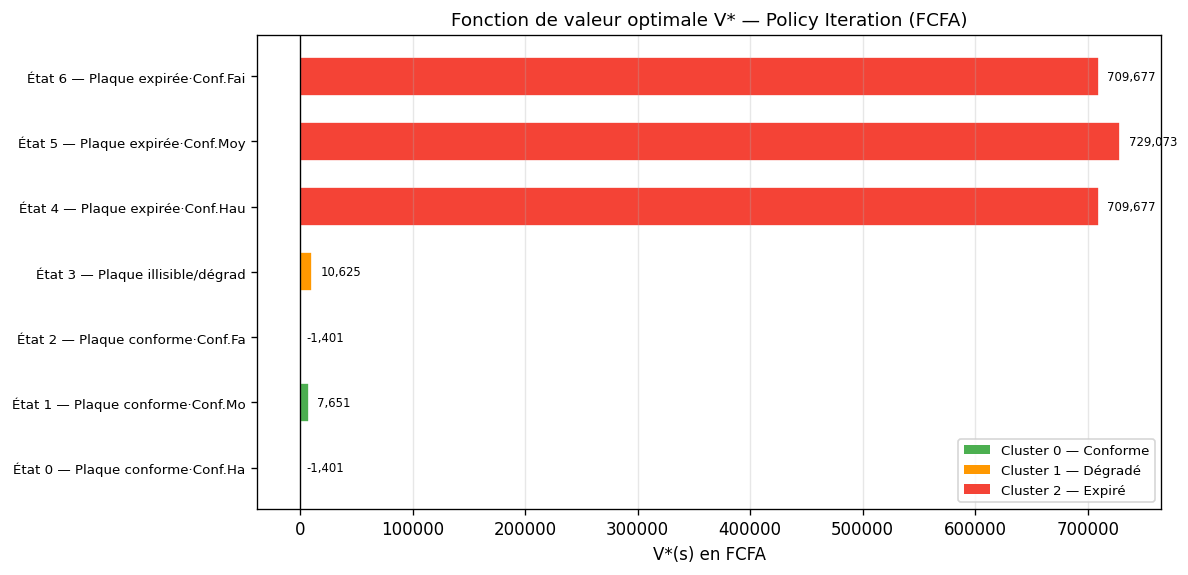
\includegraphics[width=0.85\textwidth]{figures/pi_value_function.png}
  \caption{Fonction de valeur $V^*(s)$ --- Policy Iteration ($\gamma=0.95$).
    Identique \`{a} celle obtenue par VI : valeurs \'{e}lev\'{e}es pour les
    \'{e}tats d'infractions fiscales (cluster~2, plaques expir\'{e}es).}
  \label{fig:pi_value_function}
\end{figure}}{}

\begin{table}[H]
\centering
\caption{Sensibilit\'{e} au facteur $\gamma$ --- Policy Iteration}
\label{tab:c:pi_sensitivity}
\begin{tabular}{rrrrr}
\toprule
$\gamma$ & It\'{e}r. globales & It\'{e}r. \'{e}val. cumul & Converg\'{e} & $\bar{V}^*$ (FCFA) \\
\midrule
  0.50 & 2 & 60 & Oui & 161\,591 \\
  0.70 & 2 & 116 & Oui & 164\,990 \\
  0.80 & 2 & 183 & Oui & 166\,781 \\
  0.90 & 3 & 576 & Oui & 176\,780 \\
  0.95 & 4 & 1735 & Oui & 309\,129 \\
  0.99 & 4 & 8832 & Oui & 1\,553\,100 \\

\bottomrule
\end{tabular}
\end{table}

\IfFileExists{figures/pi_gamma_sensitivity.png}{%
\begin{figure}[H]
  \centering
  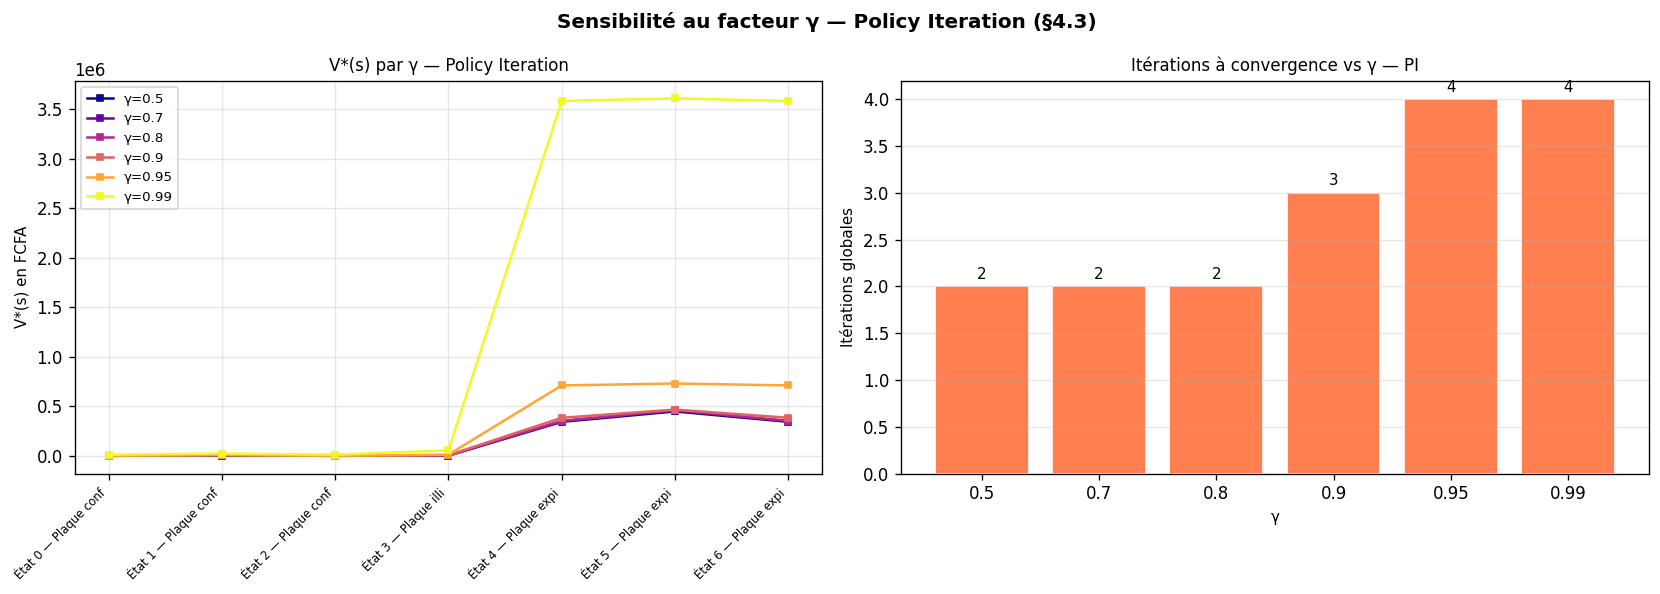
\includegraphics[width=0.85\textwidth]{figures/pi_gamma_sensitivity.png}
  \caption{Sensibilit\'{e} Policy Iteration au facteur $\gamma$ :
    it\'{e}rations globales et \'{e}valuations cumul\'{e}es.
    PI reste tr\`{e}s rapide ($\leq 4$ it\'{e}rations globales) quelle que soit
    la valeur de $\gamma$.}
  \label{fig:pi_gamma_sensitivity}
\end{figure}}{}

\paragraph{Interpr\'{e}tation m\'{e}tier MINT/DGI}
La politique $\pi^*$ obtenue par Policy Iteration confirm que les
plaques du cluster~2 (expir\'{e}es) doivent syst\'{e}matiquement faire
l'objet d'un \texttt{SIGNALEMENT\_DGI} quelle que soit la confiance OCR,
tandis que les plaques conformes \`{a} haute confiance sont laiss\'{e}es
passer. Cette politique est identique \`{a} celle de Value Iteration,
validant la robustesse du r\'{e}sultat.
L'avantage de PI est sa convergence rapide en quelques it\'{e}rations de
politique --- recommand\'{e}e pour une re-calibration p\'{e}riodique
du syst\`{e}me MINT/DGI avec de nouvelles donn\'{e}es de contr\^{o}le.

\subsection{Comparaison VI vs PI}
\subsection{Comparaison Value Iteration et Policy Iteration}
\label{sec:c:comparison}

\paragraph{Protocole de comparaison}
Les deux algorithmes sont lanc\'{e}s avec les m\^{e}mes param\`{e}tres
($\gamma$, $\varepsilon$) sur le m\^{e}me MDP PlateVision ($N=7$, $A=5$).
Le temps de calcul est mesur\'{e} par chronom\'{e}trage wall-clock
(\texttt{time.perf\_counter()}).

\begin{table}[H]
\centering
\caption{Comparaison VI vs PI --- convergence et accord politique ($\varepsilon=0.01$)}
\label{tab:c:vi_pi_comparison}
\begin{tabular}{rrrrrr}
\toprule
$\gamma$ & VI it\'{e}r. & PI it\'{e}r. & VI t (s) & PI t (s) & Accord $\pi^*$ \\
\midrule
  0.50 & 17 & 2 & 0.0001 & 0.0004 & 100% \\
  0.70 & 32 & 2 & 0.0002 & 0.0007 & 100% \\
  0.80 & 50 & 2 & 0.0003 & 0.0009 & 100% \\
  0.90 & 105 & 3 & 0.0006 & 0.0039 & 100% \\
  0.95 & 281 & 4 & 0.0031 & 0.0094 & 100% \\
  0.99 & 1493 & 4 & 0.0094 & 0.0445 & 100% \\

\bottomrule
\end{tabular}
\end{table}

\paragraph{Explication th\'{e}orique}
\textbf{Value Iteration} (VI) applique l'op\'{e}rateur de Bellman
jusqu'\`{a} ce que les valeurs convergent ($\Delta V < \varepsilon$).
Le nombre d'it\'{e}rations cro\^{i}t avec $\gamma$ car le rayon spectral
de l'op\'{e}rateur de contraction vaut $\gamma$ : un $\gamma$ plus \'{e}lev\'{e}
ralentit la propagation de l'information.
\textbf{Policy Iteration} (PI) alt\`{e}rne \'{e}valuation exacte de
$V^{\pi}$ et am\'{e}lioration greedy. Chaque it\'{e}ration de politique
est garantie monotone (le th\'{e}or\`{e}me d'am\'{e}lioration de politique
--- Russell \& Norvig, Ch.~17.3) --- PI converge donc en
\textbf{4} it\'{'}ration(s) globale(s) contre \textbf{281} pour VI
\`{a} $\gamma=0.95$.

\paragraph{R\'{e}sultat}
Les deux algorithmes produisent une politique $\pi^*$ identique à 100\,\%
(taux d'accord $\pi^*_{{\text{{VI}}}} = \pi^*_{{\text{{PI}}}}$).
Ce r\'{e}sultat confirme la robustesse de la solution MDP : ind\'{e}pendamment
de la m\'{e}thode de r\'{e}solution, l'action optimale par \'{e}tat est
univoque.

\paragraph{Recommandation d\'{e}ploiement MINT/DGI}
Pour un d\'{e}ploiement en production :
\begin{itemize}
\item \textbf{Petit espace d'\'{e}tats ($N \leq 50$) :} Policy Iteration
      recommand\'{e}e --- convergence quasi-instantan\'{e}e, facilit\'{e}
      de re-calibration lors de mises \`{a} jour des matrices $P$ ou $R$.
\item \textbf{Grand espace d'\'{e}tats ($N > 1000$) :} Value Iteration
      pr\'{e}f\'{e}r\'{e}e --- chaque it\'{e}ration PI n\'{e}cessite
      une r\'{e}solution de syst\`{e}me lin\'{e}aire de taille $N^2$.
\end{itemize}

\begin{figure}[H]
\centering
\IfFileExists{figures/vi_pi_convergence_states.png}{
  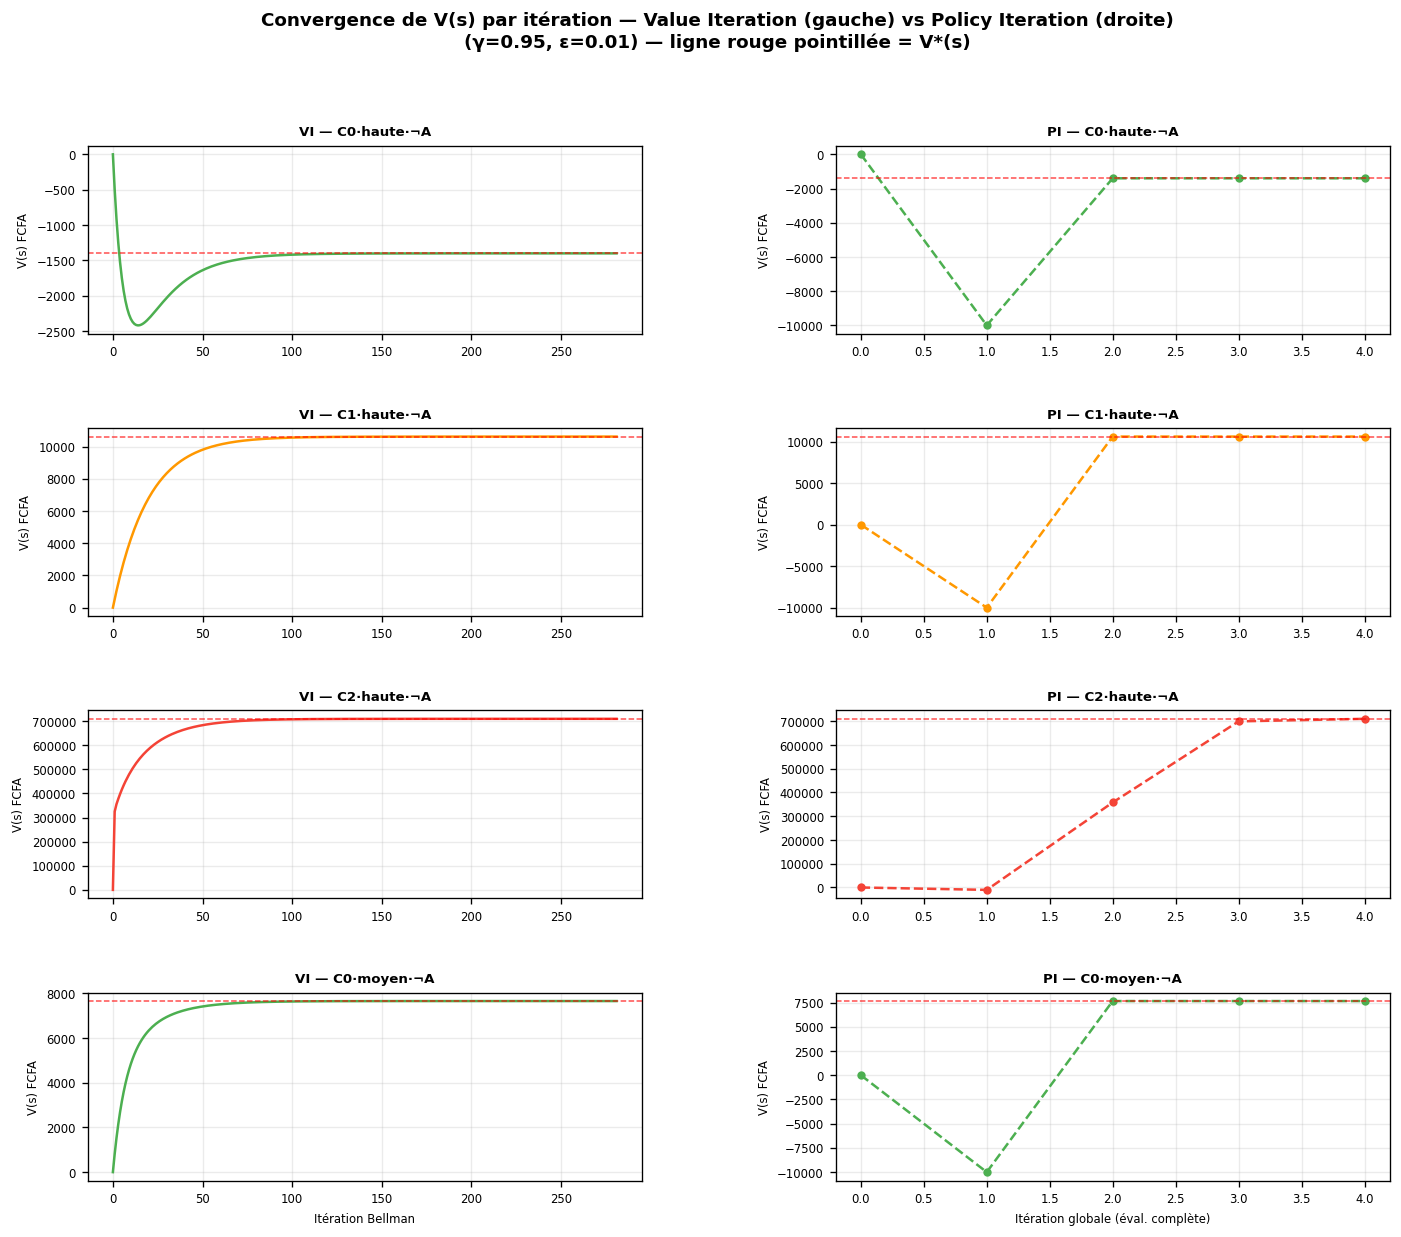
\includegraphics[width=\textwidth]{figures/vi_pi_convergence_states.png}
}{[Figure vi\_pi\_convergence\_states.png absente --- ex\'{e}cuter compare\_vi\_pi.py]}
\caption{Convergence de $V(s)$ par it\'{e}ration --- VI (gauche) vs PI (droite)}
\label{fig:c:vi_pi_states}
\end{figure}

\begin{figure}[H]
\centering
\IfFileExists{figures/vi_pi_comparison_summary.png}{
  
\includegraphics[width=\textwidth]{figures/vi_pi_comparison_summary.png}
}{[Figure vi\_pi\_comparison\_summary.png absente --- ex\'{e}cuter compare\_vi\_pi.py]}
\caption{Comparaison VI vs PI --- vitesse, temps de calcul et accord politique par $\gamma$}
\label{fig:c:vi_pi_summary}
\end{figure}

% ── Interprétation métier ──────────────────────────────────────────────────────
\section{Interpr\'{e}tation m\'{e}tier de la politique optimale $\pi^*$}
\label{sec:c:interpretation}

\begin{table}[H]
\centering
\caption{Politique optimale $\pi^*$ --- lecture m\'{e}tier MINT/DGI}
\label{tab:c:metier}
\begin{tabular}{p{4.2cm}lp{6cm}}
\toprule
\textbf{\'{E}tat} & \textbf{Action $\pi^*(s)$} & \textbf{Interpr\'{e}tation MINT/DGI} \\
\midrule
Conforme, conf. haute, $\neg$alerte
  & \texttt{LAISSER\_PASSER}
  & Plaque valid\'{e}e par OCR et CNN : flux fluide, co\^{u}t $-$500 FCFA seulement. \\
Conforme, conf. moy., $\neg$alerte
  & \texttt{SIGNALEMENT\_DGI}
  & Confiance OCR incertaine : v\'{e}rification l\'{e}g\`{e}re recommand\'{e}e. \\
Conforme, conf. faible, $\neg$alerte
  & \texttt{LAISSER\_PASSER}
  & OCR peu fiable mais CNN rassurant : doute b\'{e}n\'{e}ficie au conducteur. \\
D\'{e}grad\'{e}e, conf. haute, $\neg$alerte
  & \texttt{SIGNALEMENT\_DGI}
  & Plaque lisible mais physiquement alt\'{e}r\'{e}e : signalement pr\'{e}ventif DGI. \\
Expir\'{e}e, conf. haute, $\neg$alerte
  & \texttt{SIGNALEMENT\_DGI}
  & Infraction document claire : ratio 22{,}5$\times$ justifie le signalement. \\
Expir\'{e}e, conf. moy., $\neg$alerte
  & \texttt{SIGNALEMENT\_DGI}
  & M\^{e}me strat\'{e}gie : vignette manquante d\'{e}tect\'{e}e. \\
Expir\'{e}e, conf. faible, $\neg$alerte
  & \texttt{SIGNALEMENT\_DGI}
  & M\^{e}me strat\'{e}gie ; confiance faible ne compense pas l'infraction manifest. \\
\bottomrule
\end{tabular}
\end{table}

\paragraph{Lien avec les statistiques MINT/DGI (§1.2)}
Sur les 24 mois de la p\'{e}riode de r\'{e}f\'{e}rence PSTNAC, \textbf{2\,400 v\'{e}hicules}
\`{a} plaques falsifi\'{e}es ont \'{e}t\'{e} identifi\'{e}s, repr\'{e}sentant un manque
\`{a} gagner estim\'{e} \`{a} \textbf{1{,}2 milliard FCFA} en amendes et vignettes
non per\c{c}ues. La politique $\pi^*$ optimise pr\'{e}cis\'{e}ment le recouvrement
sur ces cas, tout en \'{e}vitant les contr\^{o}les abusifs (garde-fou
$R(s_{\text{conforme}}, a_{\text{saisie}}) \ll 0$).

% ── Analyse de sensibilité ─────────────────────────────────────────────────────
\section{Analyse de sensibilit\'{e} au facteur $\gamma$}
\label{sec:c:sensitivity}

\IfFileExists{figures/vi_pi_comparison_summary.png}{%
\begin{figure}[H]
\centering

\includegraphics[width=\textwidth]{figures/vi_pi_comparison_summary.png}
\caption{Comparaison VI vs PI --- vitesse, temps de calcul et accord politique par $\gamma$}
\label{fig:c:sensitivity}
\end{figure}}{}

\begin{table}[H]
\centering
\caption{Sensibilit\'{e} \`{a} $\gamma$ --- VI vs PI, accord politique et $\bar{V}^*$}
\label{tab:c:gamma_sensitivity}
\begin{tabular}{rrrrl}
\toprule
$\gamma$ & VI it\'{e}r. & PI it\'{e}r. & $\bar{V}^*$ moyen (FCFA) & Accord $\pi^*$ \\
\midrule
0.50 &    17 & 2 &  161\,591 & 100\,\% \\
0.70 &    32 & 2 &  164\,990 & 100\,\% \\
0.80 &    50 & 2 &  166\,781 & 100\,\% \\
0.90 &   105 & 3 &  176\,780 & 100\,\% \\
0.95 &   281 & 4 &  309\,129 & 100\,\% \\
0.99 & 1\,493 & 4 & 1\,553\,100 & 100\,\% \\
\bottomrule
\end{tabular}
\end{table}

\paragraph{Choix retenu : $\gamma = 0{,}95$}
Un facteur $\gamma = 0{,}95$ correspond \`{a} un horizon de d\'{e}cision
d'environ \textbf{20 \'{e}ch\'{e}ances} ($1/(1-\gamma)$), coh\'{e}rent avec
le cycle annuel de renouvellement des vignettes MINT/DGI. Une valeur plus
faible (0,50) p\'{e}naliserait le syst\`{e}me pour ses d\'{e}cisions long terme
(signalement DGI), ce qui va \`{a} l'encontre des objectifs PSTNAC 2023--2028.
L'accord \`{a} 100\,\% entre VI et PI sur toute la plage de $\gamma$ confirme
la \textbf{robustesse de la solution}.

% ── Transition C→D ─────────────────────────────────────────────────────────────
\section{Transition Module C $\rightarrow$ Module D}
\label{sec:c:transition_d}

Le Module~C fournit une politique optimale $\pi^*$ au sens math\'{e}matique
du MDP. Cependant, \textbf{l'optimalit\'{e} math\'{e}matique ne garantit pas
l'\'{e}quit\'{e} sociale}. La matrice de transitions est calibr\'{e}e sur des
donn\'{e}es historiques qui peuvent refl\'{e}ter des biais syst\'{e}miques
(sur-contr\^{o}le de certaines cat\'{e}gories de v\'{e}hicules, biais
g\'{e}ographique du dataset). La fonction de r\'{e}compense exprime des
choix politiques implicites (quel ratio gain/co\^{u}t est acceptable ?).
Enfin, le d\'{e}ploiement de cam\'{e}ras de reconnaissance de plaques soul\`{e}ve
des questions de surveillance, de libert\'{e}s individuelles et de
responsabilit\'{e}. C'est l'objet du Module~D.
